\PassOptionsToPackage{subsection=false}{beamerouterthememiniframes}
\documentclass{beamer}
\usepackage[italian]{babel}
\usepackage[utf8]{inputenc}
\usepackage[T1]{fontenc}
\usepackage{textcomp}
\usepackage{listings}
\usepackage{tabu}
\usepackage{color}


\usetheme{Ilmenau}


\title{Large Scale Data Engineering - Assignment 2}
\subtitle{Flight Routes}
\author[Group 01]{Davide Dal Bianco 2598719 \\ Filippo Sestini 2598712}
\date{10\textsuperscript{th} October 2016}
\usenavigationsymbolstemplate{}


\begin{document}

    \begin{frame}
        \maketitle
    \end{frame}

    \begin{frame}
        \frametitle{The Project}
        \begin{itemize}
            \item Analyzing air traffic
            \item Detecting standard routes
            \item Questions
            \begin{itemize}
                \item Fuel saving
                \item Abnormal routes
            \end{itemize}
            \item Tools we use
            \begin{itemize}
                \item Spark
                \item Scala
            \end{itemize}
        \end{itemize}
    \end{frame}

    \begin{frame}
        \frametitle{OpenSky Network}
        \begin{columns}
            \begin{column}{0.5\textwidth}
                
\includegraphics[width=\linewidth]{img/opensky-logo}
                \vspace*{3mm}
                \begin{itemize}
                    \item Recently born
                    \item Data collected by volunteers                    
                \end{itemize}
            \end{column}
            \begin{column}{0.5\textwidth}
                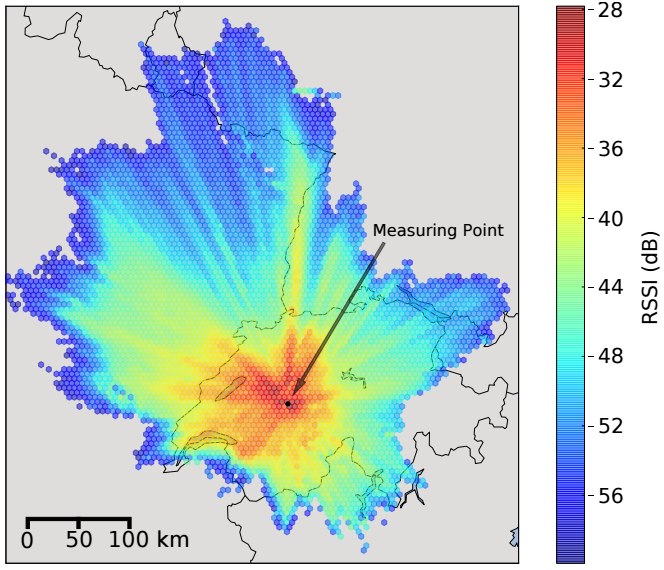
\includegraphics[width=\linewidth]{img/signal-intensity}
            \end{column}
        \end{columns}
        \vspace*{10mm}
        \textit{M. Schäfer et al., Bringing Up OpenSky: A Large-scale ADS-B Sensor Network for Research, 2014}
    \end{frame}

    \begin{frame}
        \frametitle{Dataset analysis}
        \begin{columns}
            \begin{column}{0.5\textwidth}
                \begin{itemize}
                    \item About 20 sensors
                    \begin{itemize}
                        \item $\sim 40\%$ position messages
                        \item $\sim 40\%$ velocity messages
                    \end{itemize}
                    \item About 1 billion messages
                    \item Many uncovered areas
                \end{itemize}
            \end{column}
            \begin{column}{0.5\textwidth}
                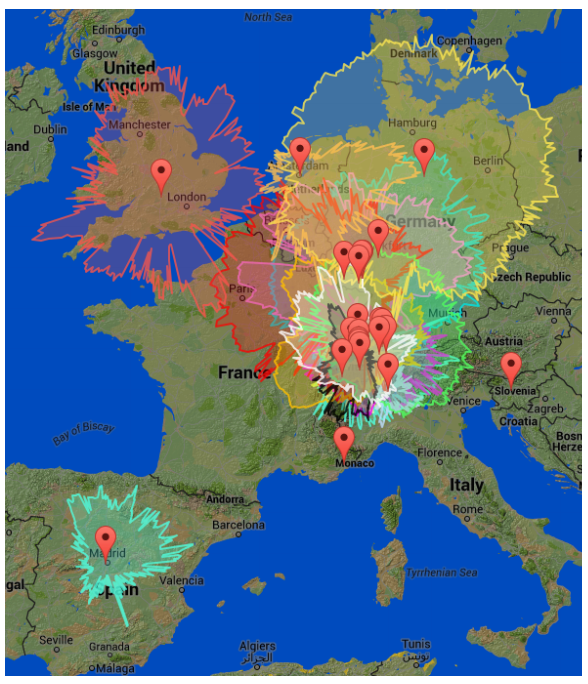
\includegraphics[width=\linewidth]{img/sensors-area}
            \end{column}
        \end{columns}
    \end{frame}

    \begin{frame}
        \frametitle{Routes detection}
        \begin{columns}
            \begin{column}{0.5\textwidth}
                \begin{itemize}
                    \item<+-> External airport dataset
                    \item<+-> Flights recognition
                    \begin{itemize}
                        \item<+-> Separation
                        \item<+-> Filtering
                        \item<+-> Detection of departure and arrival airports
                    \end{itemize}
                    \item<+-> Routes identification
                    \begin{itemize}
                        \item<.-> Aggregative clustering algorithm
                    \end{itemize}
                \end{itemize}
            \end{column}
            \begin{column}{0.5\textwidth}
                \includegraphics<1>[width=\linewidth]{img/airports}
                \includegraphics<2>[width=\linewidth]{img/altitudes}
                \includegraphics<3>[width=\linewidth]{img/altitudes-marked}
                \includegraphics<4,5>[width=\linewidth]{img/altitudes-filtered}
                \includegraphics<6>[width=\linewidth]{img/routes-clustering}
            \end{column}
        \end{columns}
        \vspace*{10mm}
        \only<6>{\textit{James S. DeArmon et al., Air Route Clustering for a Queuing Network Model of the National Airspace System, 2014}}
    \end{frame}

    \begin{frame}
        \frametitle{To do}
        \begin{itemize}
            \item Updated dataset
            \item Clustering parameters
            \item Deployment
            \item Data visualization
        \end{itemize}
    \end{frame}

\end{document}


